\documentclass{beamer}
%
% Choose how your presentation looks.
%
% For more themes, color themes and font themes, see:
% http://deic.uab.es/~iblanes/beamer_gallery/index_by_theme.html
%
\usetheme[style=simple,nat]{Frederiksberg}
\usefonttheme{serif}
\usepackage{tikz}
\usepackage{Nikolai}
\usepackage[english]{babel}
\usepackage[super]{nth}

\newcommand{\coef}[1]{_{[#1]}}


\title{Visualisation of Concepts in Condensed Matter Physics}
\author{Nikolai Plambech Nielsen}
\institute{Niels Bohr Institute}
\date{\nth{27} of June, 2018}

\begin{document}

\begin{frame}
  \titlepage
  Supervised by Mark Spencer Rudner
\end{frame}


\section{Outline}
\begin{frame}{Outline}
\begin{itemize}
  \item Introduction / Background
  \item Lattices and crystal structure
  \item The reciprocal lattice and scattering
  \item Band structure
  \item Discussion
\end{itemize}
\end{frame}


\section{Introduction / Background}
\begin{frame}{Introduction / Background}
\onslide<1->{Periodic medium. Discrete translational symmetry}
\begin{equation*}
	\onslide<2->{[\op{T}_{\V{R}}, \op{H}]=0, \quad  V(\V{r}+\V{R}) = V(\V{r}),}
\end{equation*}
\onslide<3->{Bloch's theorem:}
\begin{align*}
	\onslide<3->{\psi(\V{r}) &= e^{i \V{k}\D \V{r}} u(\V{r}), \quad u(\V{r}+\V{R}) = u(\V{r}),} \\
	\onslide<4->{&= \sum_{\V{G}} u_{\V{G},\V{k}} e^{i (\V{G}+\V{k}) \D \V{r}}.}
\end{align*}
\onslide<5->{Crystal momentum. One dimension, spacing of $ a $:}
\begin{equation*}
	\onslide<6->{k \to k+\frac{2\pi}{a}, \quad -\frac{\pi}{a} \leq k \leq \frac{\pi}{a}}
\end{equation*}
\end{frame}

\begin{frame}{Lattices and crystal structure}
\begin{equation*}
\onslide<2->{\V{R} = \sum_{i = 1}^{d} n_i \V{a}_i, \quad n_i \in \mathbb{Z}}
\end{equation*}
\begin{figure}[H]
	\centering
	\begin{minipage}{.4\textwidth}
		\centering
		\begin{tikzpicture}
			\node<2> (img1) {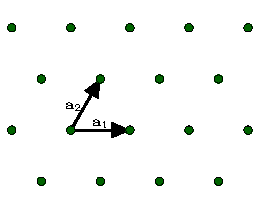
\includegraphics[width=\linewidth]{figures/triangular.pdf}};
			\node<3> (img2) {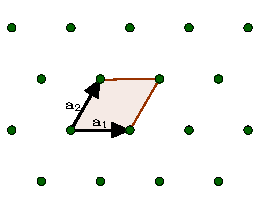
\includegraphics[width=\linewidth]{figures/triangularUnit.pdf}};
		\end{tikzpicture}
		\onslide<2->{\captionof{figure}{A triangular lattice. $ \V{a}_1 = a\D(1,0)$, \\$\V{a}_2 = a\D(1/2, \sqrt{3}/2) $.}}
		\label{fig:triangular_unitcell}
	\end{minipage}%
	\hfill
	\begin{minipage}{.4\textwidth}
		\centering
		\begin{tikzpicture}
			\node<2> (img3) {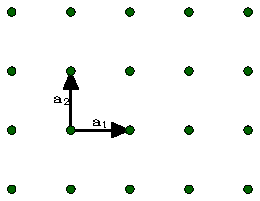
\includegraphics[width=\linewidth]{figures/square.pdf}};
			\node<3> (img4) {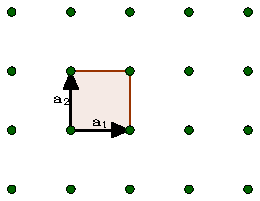
\includegraphics[width=\linewidth]{figures/squareUnit.pdf}};
		\end{tikzpicture}
		\onslide<2->{\captionof{figure}{A square lattice. $ \V{a}_1 = a\D(1,0), \V{a}_2 = a\D(0,1) $.}}
		\label{fig:square_unitcell}
	\end{minipage}
\end{figure}
\end{frame}

\begin{frame}{Lattices and crystal structure}
\pause
\begin{equation*}
	\V{r}_{atom,i} = \V{R} + \V{r}_{basis, i},
\end{equation*}
\pause
\begin{figure}[H]
	\centering
	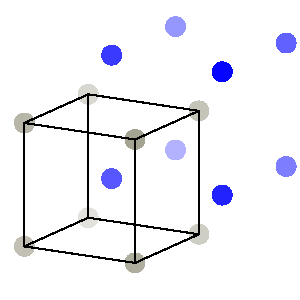
\includegraphics{figures/lattice_unfinished_1.pdf}
	\caption{Conventional unit cell of a bcc lattice. Two atoms, one (grey) at $ a \D (0,0,0) $ and one (blue) at $ a\D(1/2, 1/2, 1/2) $.}
\end{figure}
\end{frame}

\begin{frame}{Lattices and crystal structure}
\begin{figure}[H]
	\centering
	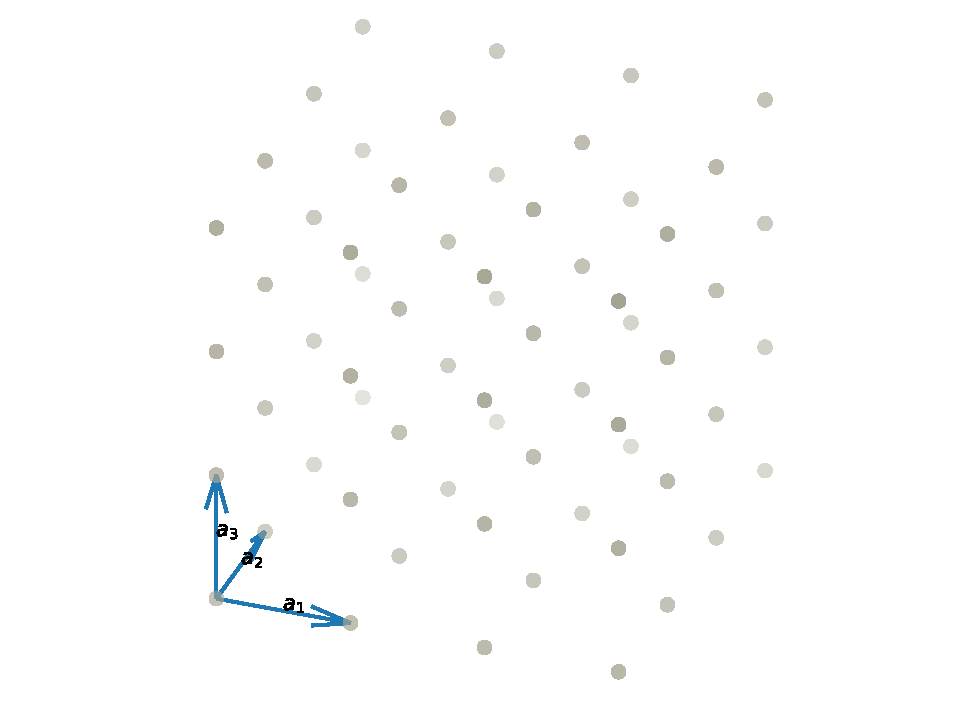
\includegraphics[width=.7\linewidth]{figures/cubic_no_grid.pdf}
	\caption{A simple cubic lattice. $ \V{a}_1 = a\D (1,0,0), \V{a}_2 = a\D(0,1,0), \V{a}_3 = a\D (0,0,1) $.}
	\label{fig:cubic_no_grid}
\end{figure}
\end{frame}

\begin{frame}{Lattices and crystal structure}
\begin{figure}[H]
	\centering
	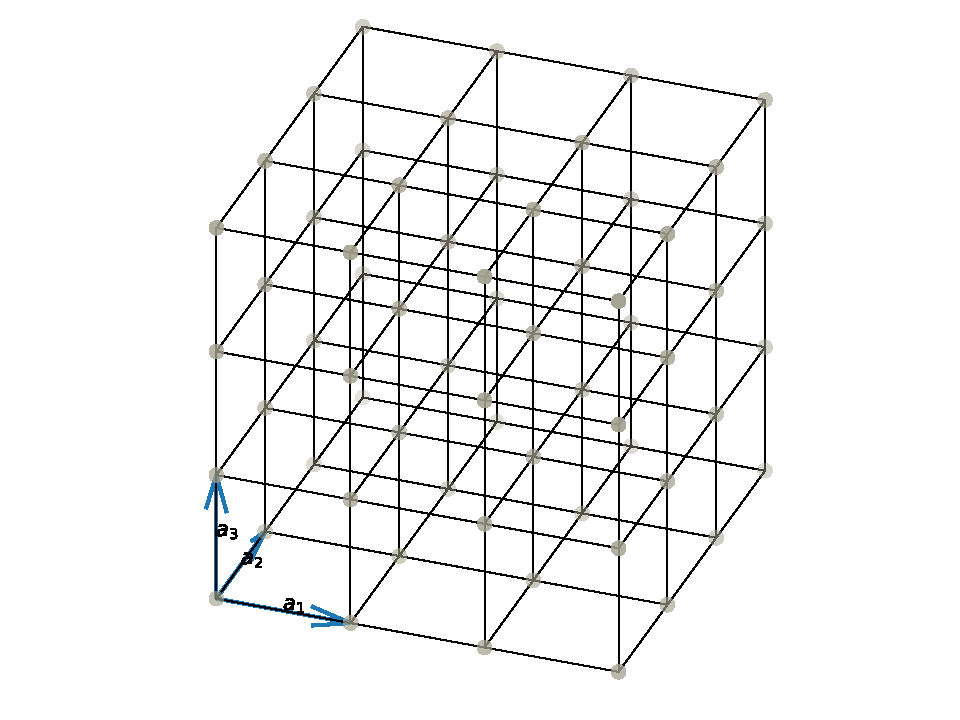
\includegraphics[width=.7\linewidth]{figures/cubic_grid.pdf}
	\caption{A simple cubic lattice. $ \V{a}_1 = a\D (1,0,0), \V{a}_2 = a\D(0,1,0), \V{a}_3 = a\D (0,0,1) $.}
	\label{fig:cubic_grid}
\end{figure}
\end{frame}


\begin{frame}{Lattices and crystal structure}
\end{frame}


\section{Reciprocal lattice and scattering}
\begin{frame}{Reciprocal lattice and scattering}
\begin{equation*}
	e^{i \V{G} \D\V{R}} = 1,
\end{equation*}
\begin{equation*}
	\V{G} = h \V{b}_1 + k\V{b}_2 + l\V{b}_3, \quad h,k,l \in \mathbb{Z}
\end{equation*}
\begin{equation*}
	\V{a}_i \D \V{b}_j = 2\pi \delta_{ij},
\end{equation*}
\end{frame}

\begin{frame}{Reciprocal lattice and scattering}
Free particles:
\begin{equation*}
	E_{\V{k}} = \frac{\hbar^2 \V{k}^2}{2m},
\end{equation*}
Fermi's Golden Rule
\begin{align*}
	\Gamma(\V{k}', \V{k}) &= \frac{2\pi}{\hbar}|\braket{\V{k}' | V | \V{k}}|^2 \delta(E_{\V{k}'}-E_{\V{k}}), \\
	\braket{\V{k}' | V | \V{k}} &= \infint \frac{e^{-i \V{k}'\D\V{r}}}{\sqrt{L^3}} V(\V{r}) \frac{e^{i \V{k}\D\V{r}}}{\sqrt{L^3}} \ud \V{r}, \\
	&= \frac{1}{L^3} \infint e^{-i(\V{k}'-\V{k}) \D \V{r}} \, V(\V{r}) \ud \V{r}.
\end{align*}
\end{frame}

\begin{frame}{Reciprocal lattice and scattering}
\begin{equation*}
	\V{r} = \V{R} + \V{x},
\end{equation*} 
\begin{align*}
	\braket{\V{k}' | V | \V{k}} &= \frac{1}{L^3} \sum_{\V{R}} e^{-i(\V{k}'-\V{k}) \D\V{R}} S(\V{k}'-\V{k}), \\
	S(\V{k}'-\V{k}) &=  \int_{\substack{\text{unit-} \\\text{cell}}} e^{-i (\V{k}'-\V{k}) \D \V{x}} V(\V{x}) \ud \V{x}, \\
	\sum_{\V{R}} e^{-i (\V{k}'-\V{k}) \D \V{R}} &= \begin{cases}
	N, & \V{k}'-\V{k} = \V{G}, \\
	0, & \V{k}'-\V{k} \neq \V{G}.
	\end{cases}
\end{align*}
\end{frame}

\begin{frame}{Reciprocal lattice and scattering}
\begin{equation*}
	\V{k}'-\V{k} = \V{G}, \quad |\V{k}| = |\V{k}'|,
\end{equation*}
\begin{equation*}
	I \propto |S(\V{G})|^2.
\end{equation*}
\end{frame}

\begin{frame}{Reciprocal lattice and scattering}
Neutron scattering
\begin{equation*}
	V(\V{x}) = \sum_{\text{atoms } j} f_j \, \delta(\V{x}-\V{x}_j), \quad S(\V{G}) = \sum_{\text{atoms } j} f_j e^{i\V{G} \D \V{x}_j}
\end{equation*}
\end{frame}

\begin{frame}{Reciprocal lattice and scattering}
Systemic absences
\begin{equation*}
	S(\V{G}) = S_{hkl} = \sum_{\text{atoms } j} f_j e^{2\pi i(hx_j + ky_j + lz_j)}
\end{equation*}
bcc ($ h+k+l $ even)
\begin{equation*}
	S_{hkl} = f (1+ (-1)^{h+k+l})
\end{equation*}
fcc ($ h,k,l $ all either even or odd)
\begin{equation*}
	S_{hkl} = f (1+ e^{\pi i(h+k)} + e^{\pi i(k+l)} + e^{\pi i(h+l)})
\end{equation*}
\end{frame}

\begin{frame}{Reciprocal lattice and scattering}
\end{frame}


\section{Band structure}
\begin{frame}{Band structure}
	2 dimensional square lattice.
	\begin{figure}[H]
		\centering
		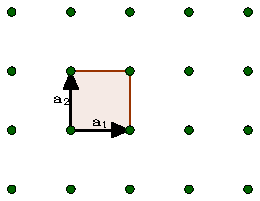
\includegraphics[width=0.5\linewidth]{figures/squareUnit.pdf}
		\captionof{figure}{A square lattice. $ \V{a}_1 = a\D(1,0), \V{a}_2 = a\D(0,1) $.}
		\label{fig:band_structure_lattice}
	\end{figure}
	First Brillouin zone: $ -\pi/a \leq k_i \leq \pi/a $
\end{frame}

\begin{frame}{Band structure}
Fourier transform the Schrödinger equation.
\begin{align*}\label{key}
	V(\V{r}+\V{R}) &= V(\V{r}) \quad \Leftrightarrow \quad V(\V{r}) = \sum_{\V{G}} V_{\V{G}} e^{i\V{G} \D \V{r}},\\
	V_{\V{G}} &= \frac{1}{a^2}\int_{\substack{\text{unit-} \\\text{cell}}} e^{-i (\V{k}'-\V{k}) \D \V{x}} V(\V{x}) \ud \V{x},
\end{align*}
\begin{equation*}\label{key}
	\sum_{\V{G}} \bb{\frac{\hbar^2 \V{k}^2}{2m} \delta_{\V{G},0} + V_{\V{G}} } \tilde{\psi}(\V{k}-\V{G}) = E \tilde{\psi} (\V{k})
\end{equation*}
\end{frame}

\begin{frame}{Band structure}
Matrix equation and notation.
\begin{align*}
V_{\V{G}} &= V\coef{m_1, m_2}, \quad \V{G} = m_1 \V{b}_1 + m_2 \V{b}_2, \\
\ket{\psi} &= \begin{pmatrix}
\vdots \\ \tilde{\psi}(\V{k}-\V{G}_1) \\ \tilde{\psi}(\V{k}) \\ \tilde{\psi}(\V{k}+\V{G}_1) \\ \vdots
\end{pmatrix} = \begin{pmatrix}
\vdots \\ \psi\coef{0, -1}\\ \psi\coef{0, 0} \\ \psi\coef{0, 1} \\ \vdots
\end{pmatrix}, \\
T &= \frac{\hbar^2}{2m} \begin{pmatrix}
\ddots	& 		 			&			& 					& \\
& (\V{k}-\V{G}_1)^2	& 			& 					& \\
& 	 				& \V{k}^2	& 					& \\
&					&			& (\V{k}+\V{G}_1)^2	& \\
&					&			&					& \ddots
\end{pmatrix}.
\end{align*}
\begin{equation*}
\end{equation*}
\end{frame}

\begin{frame}{Band structure}
\begin{align*}
[m_1, m_2] \in \{ &[-1, -1], [-1, 0], [-1, 1],\\ &[0, -1], [0, 0], [0, 1],\\ &[1,-1], [1, 0], [1,1]  \}.
\end{align*}
\begin{align*}
E \psi\coef{-1,0} = {} & \sum_{m'_1 =  -\infty}^{\infty}\sum_{m'_2 = -\infty}^{\infty} V\coef{m'_1, m'_2} \ \psi\coef{-1-m'_1, -m'_2}, \\
= {} & \dots +  V\coef{-2, -1}\psi\coef{1,1} + V\coef{-2, 0} \psi\coef{1, 0} + V\coef{-2, 1}\psi\coef{1,-1} +  \dots  \\
& + V\coef{-1, -1} \psi\coef{-2, 1} + V\coef{-1, 0} \psi\coef{-2, 0} + V\coef{-1, 1} \psi\coef{-2, -1} + \dots\\
& + V\coef{0, -1} \psi\coef{-1, 1} + V\coef{0, 0} \psi\coef{-1, 0} + V\coef{0, 1}\psi\coef{-1, -1} + \dots\\
&+ V\coef{1, -1} \psi \coef{0,1} + V\coef{1, 0} \psi \coef{0, 0} + V\coef{1,1} \psi \coef{0, -1} + \dots.
\end{align*}
\end{frame}

\begin{frame}{Band structure}
\begin{align*}
[m_1, m_2] \in \{ &[-1, -1], [-1, 0], [-1, 1],\\ &[0, -1], [0, 0], [0, 1],\\ &[1,-1], [1, 0], [1,1]  \}.
\end{align*}
Row $ [m_1, m_2] $ , column $ [m_1', m_2'] $: $ V\coef{m_1-m'_1, m_2-m'_2} $ .
\end{frame}

\begin{frame}{Band structure}
\begin{align*}\label{key}
	V_{\text{dirac}}(\V{r}) &= V_0 a^2 \sum_{\V{R}} \delta(\V{r}-\V{R}), \quad V_{\text{dirac},\V{G}} = V_0, \\
	V_{\text{harmonic}}(\V{r}) &= V_0 \bb{\cos\pp{\frac{2\pi}{a} x} + \cos\pp{\frac{2\pi}{a} y}},\\
	V_{\text{harmonic}, \V{G}} &= \begin{cases}
	\frac{V_0}{2} 	& \text{if } [m_1, m_2] \in \{[0,1], [0,-1], [1,0], [-1,0]\}, \\
	0					& \text{else}.
	\end{cases}
\end{align*}
\end{frame}

\begin{frame}{Band structure}
\begin{equation*}
V_{\text{harmonic}} = \frac{V_0}{2} \begin{pmatrix}
0 & 1 & 0 & 1 & 0 & 0 & 0 & 0 & 0 \\
1 & 0 & 1 & 0 & 1 & 0 & 0 & 0 & 0 \\
0 & 1 & 0 & 0 & 0 & 1 & 0 & 0 & 0 \\
1 & 0 & 0 & 0 & 1 & 0 & 1 & 0 & 0 \\
0 & 1 & 0 & 1 & 0 & 1 & 0 & 1 & 0 \\
0 & 0 & 1 & 0 & 1 & 0 & 0 & 0 & 1 \\
0 & 0 & 0 & 1 & 0 & 0 & 0 & 1 & 0 \\
0 & 0 & 0 & 0 & 1 & 0 & 1 & 0 & 1 \\
0 & 0 & 0 & 0 & 0 & 1 & 0 & 1 & 0
\end{pmatrix}.
\end{equation*}
\end{frame}

\begin{frame}{Band structure}
Define $ k_0 \equiv 2\pi/a, E_0 \equiv \hbar^2 k_0^2/m $:
\begin{equation*}
	\sum_{\tilde{\V{G}}} \bb{\frac{\tilde{\V{k}}^2}{2} \delta_{\tilde{\V{G}},0} + \tilde{V}_{\tilde{\V{G}}}} \tilde{\psi}(\tilde{\V{k}} - \tilde{\V{G}}) = \tilde{E} \tilde{\psi}(\tilde{\V{k}}),
\end{equation*}
\begin{align*}
	\tilde{\V{G}} &\equiv \V{G}/k_0 = m_1 \U{x}+m_2 \U{y}, \\
	\tilde{\V{k}} &\equiv \V{k}/k_0, \quad -\frac{1}{2} \leq \tilde{\V{k}}_x \leq \frac{1}{2}\\
	\tilde{V}_{\tilde{\V{G}}} &\equiv V_{\V{G}} / E_0, \quad \tilde{E} \equiv E/E_0
\end{align*}
\end{frame}

\begin{frame}{Band structure}
\end{frame}



\section{Discussion}
\begin{frame}{Discussion}
\begin{itemize}
	\item 3 (4) programs
	\begin{itemize}
		\item Lattice plotting
		\item (Plotting of Lattice planes)
		\item Scattering simulation
		\item Band structure of 2D materials
	\end{itemize}
	\item command line interface - convert to graphical user interface
	\item Problems with Matplotlib
\end{itemize}
\end{frame}

\end{document}
